\documentclass[1p]{elsarticle_modified}
%\bibliographystyle{elsarticle-num}

%\usepackage[colorlinks]{hyperref}
%\usepackage{abbrmath_seonhwa} %\Abb, \Ascr, \Acal ,\Abf, \Afrak
\usepackage{amsfonts}
\usepackage{amssymb}
\usepackage{amsmath}
\usepackage{amsthm}
\usepackage{scalefnt}
\usepackage{amsbsy}
\usepackage{kotex}
\usepackage{caption}
\usepackage{subfig}
\usepackage{color}
\usepackage{graphicx}
\usepackage{xcolor} %% white, black, red, green, blue, cyan, magenta, yellow
\usepackage{float}
\usepackage{setspace}
\usepackage{hyperref}

\usepackage{tikz}
\usetikzlibrary{arrows}

\usepackage{multirow}
\usepackage{array} % fixed length table
\usepackage{hhline}

%%%%%%%%%%%%%%%%%%%%%
\makeatletter
\renewcommand*\env@matrix[1][\arraystretch]{%
	\edef\arraystretch{#1}%
	\hskip -\arraycolsep
	\let\@ifnextchar\new@ifnextchar
	\array{*\c@MaxMatrixCols c}}
\makeatother %https://tex.stackexchange.com/questions/14071/how-can-i-increase-the-line-spacing-in-a-matrix
%%%%%%%%%%%%%%%

\usepackage[normalem]{ulem}

\newcommand{\msout}[1]{\ifmmode\text{\sout{\ensuremath{#1}}}\else\sout{#1}\fi}
%SOURCE: \msout is \stkout macro in https://tex.stackexchange.com/questions/20609/strikeout-in-math-mode

\newcommand{\cancel}[1]{
	\ifmmode
	{\color{red}\msout{#1}}
	\else
	{\color{red}\sout{#1}}
	\fi
}

\newcommand{\add}[1]{
	{\color{blue}\uwave{#1}}
}

\newcommand{\replace}[2]{
	\ifmmode
	{\color{red}\msout{#1}}{\color{blue}\uwave{#2}}
	\else
	{\color{red}\sout{#1}}{\color{blue}\uwave{#2}}
	\fi
}

\newcommand{\Sol}{\mathcal{S}} %segment
\newcommand{\D}{D} %diagram
\newcommand{\A}{\mathcal{A}} %arc


%%%%%%%%%%%%%%%%%%%%%%%%%%%%%5 test

\def\sl{\operatorname{\textup{SL}}(2,\Cbb)}
\def\psl{\operatorname{\textup{PSL}}(2,\Cbb)}
\def\quan{\mkern 1mu \triangleright \mkern 1mu}

\theoremstyle{definition}
\newtheorem{thm}{Theorem}[section]
\newtheorem{prop}[thm]{Proposition}
\newtheorem{lem}[thm]{Lemma}
\newtheorem{ques}[thm]{Question}
\newtheorem{cor}[thm]{Corollary}
\newtheorem{defn}[thm]{Definition}
\newtheorem{exam}[thm]{Example}
\newtheorem{rmk}[thm]{Remark}
\newtheorem{alg}[thm]{Algorithm}

\newcommand{\I}{\sqrt{-1}}
\begin{document}

%\begin{frontmatter}
%
%\title{Boundary parabolic representations of knots up to 8 crossings}
%
%%% Group authors per affiliation:
%\author{Yunhi Cho} 
%\address{Department of Mathematics, University of Seoul, Seoul, Korea}
%\ead{yhcho@uos.ac.kr}
%
%
%\author{Seonhwa Kim} %\fnref{s_kim}}
%\address{Center for Geometry and Physics, Institute for Basic Science, Pohang, 37673, Korea}
%\ead{ryeona17@ibs.re.kr}
%
%\author{Hyuk Kim}
%\address{Department of Mathematical Sciences, Seoul National University, Seoul 08826, Korea}
%\ead{hyukkim@snu.ac.kr}
%
%\author{Seokbeom Yoon}
%\address{Department of Mathematical Sciences, Seoul National University, Seoul, 08826,  Korea}
%\ead{sbyoon15@snu.ac.kr}
%
%\begin{abstract}
%We find all boundary parabolic representation of knots up to 8 crossings.
%
%\end{abstract}
%\begin{keyword}
%    \MSC[2010] 57M25 
%\end{keyword}
%
%\end{frontmatter}

%\linenumbers
%\tableofcontents
%
\newcommand\colored[1]{\textcolor{white}{\rule[-0.35ex]{0.8em}{1.4ex}}\kern-0.8em\color{red} #1}%
%\newcommand\colored[1]{\textcolor{white}{ #1}\kern-2.17ex	\textcolor{white}{ #1}\kern-1.81ex	\textcolor{white}{ #1}\kern-2.15ex\color{red}#1	}

{\Large $\underline{11n_{29}~(K11n_{29})}$}

\setlength{\tabcolsep}{10pt}
\renewcommand{\arraystretch}{1.6}
\vspace{1cm}\begin{tabular}{m{100pt}>{\centering\arraybackslash}m{274pt}}
\multirow{5}{120pt}{
	\centering
	\includegraphics[width=112pt]{../../../GIT/diagram.site/Diagrams/png/645_11n_29.png}\\
\ \ \ A knot diagram\footnotemark}&
\allowdisplaybreaks
\textbf{Linearized knot diagam} \\
\cline{2-2}
 &
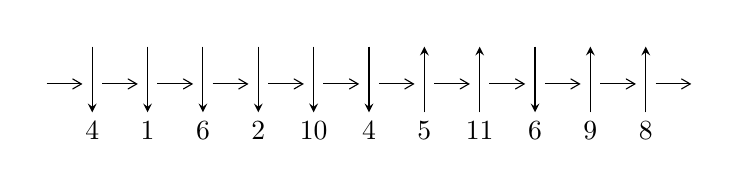
\begin{tikzpicture}[x=20pt, y=17pt]
	% nodes
	\node (C0) at (0, 0) {};
	\node (C1) at (1, 0) {};
	\node (C1U) at (1, +1) {};
	\node (C1D) at (1, -1) {4};

	\node (C2) at (2, 0) {};
	\node (C2U) at (2, +1) {};
	\node (C2D) at (2, -1) {1};

	\node (C3) at (3, 0) {};
	\node (C3U) at (3, +1) {};
	\node (C3D) at (3, -1) {6};

	\node (C4) at (4, 0) {};
	\node (C4U) at (4, +1) {};
	\node (C4D) at (4, -1) {2};

	\node (C5) at (5, 0) {};
	\node (C5U) at (5, +1) {};
	\node (C5D) at (5, -1) {10};

	\node (C6) at (6, 0) {};
	\node (C6U) at (6, +1) {};
	\node (C6D) at (6, -1) {4};

	\node (C7) at (7, 0) {};
	\node (C7U) at (7, +1) {};
	\node (C7D) at (7, -1) {5};

	\node (C8) at (8, 0) {};
	\node (C8U) at (8, +1) {};
	\node (C8D) at (8, -1) {11};

	\node (C9) at (9, 0) {};
	\node (C9U) at (9, +1) {};
	\node (C9D) at (9, -1) {6};

	\node (C10) at (10, 0) {};
	\node (C10U) at (10, +1) {};
	\node (C10D) at (10, -1) {9};

	\node (C11) at (11, 0) {};
	\node (C11U) at (11, +1) {};
	\node (C11D) at (11, -1) {8};
	\node (C12) at (12, 0) {};

	% arrows
	\draw[->,>={angle 60}]
	(C0) edge (C1) (C1) edge (C2) (C2) edge (C3) (C3) edge (C4) (C4) edge (C5) (C5) edge (C6) (C6) edge (C7) (C7) edge (C8) (C8) edge (C9) (C9) edge (C10) (C10) edge (C11) (C11) edge (C12) ;	\draw[->,>=stealth]
	(C1U) edge (C1D) (C2U) edge (C2D) (C3U) edge (C3D) (C4U) edge (C4D) (C5U) edge (C5D) (C6U) edge (C6D) (C7D) edge (C7U) (C8D) edge (C8U) (C9U) edge (C9D) (C10D) edge (C10U) (C11D) edge (C11U) ;
	\end{tikzpicture} \\
\hhline{~~} \\& 
\textbf{Solving Sequence} \\ \cline{2-2} 
 &
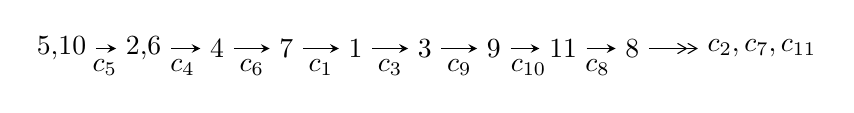
\begin{tikzpicture}[x=25pt, y=7pt]
	% node
	\node (A0) at (-1/8, 0) {5,10};
	\node (A1) at (17/16, 0) {2,6};
	\node (A2) at (17/8, 0) {4};
	\node (A3) at (25/8, 0) {7};
	\node (A4) at (33/8, 0) {1};
	\node (A5) at (41/8, 0) {3};
	\node (A6) at (49/8, 0) {9};
	\node (A7) at (57/8, 0) {11};
	\node (A8) at (65/8, 0) {8};
	\node (C1) at (1/2, -1) {$c_{5}$};
	\node (C2) at (13/8, -1) {$c_{4}$};
	\node (C3) at (21/8, -1) {$c_{6}$};
	\node (C4) at (29/8, -1) {$c_{1}$};
	\node (C5) at (37/8, -1) {$c_{3}$};
	\node (C6) at (45/8, -1) {$c_{9}$};
	\node (C7) at (53/8, -1) {$c_{10}$};
	\node (C8) at (61/8, -1) {$c_{8}$};
	\node (A9) at (10, 0) {$c_{2},c_{7},c_{11}$};

	% edge
	\draw[->,>=stealth]	
	(A0) edge (A1) (A1) edge (A2) (A2) edge (A3) (A3) edge (A4) (A4) edge (A5) (A5) edge (A6) (A6) edge (A7) (A7) edge (A8) ;
	\draw[->>,>={angle 60}]	
	(A8) edge (A9);
\end{tikzpicture} \\ 

\end{tabular} \\

\footnotetext{
The image of knot diagram is generated by the software ``\textbf{Draw programme}" developed by Andrew Bartholomew(\url{http://www.layer8.co.uk/maths/draw/index.htm\#Running-draw}), where we modified some parts for our purpose(\url{https://github.com/CATsTAILs/LinksPainter}).
}\phantom \\ \newline 
\centering \textbf{Ideals for irreducible components\footnotemark of $X_{\text{par}}$} 
 
\begin{align*}
I^u_{1}&=\langle 
u^{27}- u^{26}+\cdots+b+2 u,\;u^{25}- u^{24}+\cdots+a-2,\;u^{29}-2 u^{28}+\cdots+3 u-1\rangle \\
I^u_{2}&=\langle 
b+1,\;- u^2+a- u,\;u^4+u^3+u^2+1\rangle \\
\\
\end{align*}
\raggedright * 2 irreducible components of $\dim_{\mathbb{C}}=0$, with total 33 representations.\\
\footnotetext{All coefficients of polynomials are rational numbers. But the coefficients are sometimes approximated in decimal forms when there is not enough margin.}
\newpage
\renewcommand{\arraystretch}{1}
\centering \section*{I. $I^u_{1}= \langle u^{27}- u^{26}+\cdots+b+2 u,\;u^{25}- u^{24}+\cdots+a-2,\;u^{29}-2 u^{28}+\cdots+3 u-1 \rangle$}
\flushleft \textbf{(i) Arc colorings}\\
\begin{tabular}{m{7pt} m{180pt} m{7pt} m{180pt} }
\flushright $a_{5}=$&$\begin{pmatrix}1\\0\end{pmatrix}$ \\
\flushright $a_{10}=$&$\begin{pmatrix}0\\u\end{pmatrix}$ \\
\flushright $a_{2}=$&$\begin{pmatrix}- u^{25}+u^{24}+\cdots-3 u+2\\- u^{27}+u^{26}+\cdots+2 u^2-2 u\end{pmatrix}$ \\
\flushright $a_{6}=$&$\begin{pmatrix}1\\u^2\end{pmatrix}$ \\
\flushright $a_{4}=$&$\begin{pmatrix}- u^{27}+u^{26}+\cdots-4 u+3\\- u^{27}+u^{26}+\cdots+u^2- u\end{pmatrix}$ \\
\flushright $a_{7}=$&$\begin{pmatrix}- u^7-2 u^3\\u^7+u^5+2 u^3+u\end{pmatrix}$ \\
\flushright $a_{1}=$&$\begin{pmatrix}- u^7-2 u^3\\- u^9- u^7-3 u^5-2 u^3- u\end{pmatrix}$ \\
\flushright $a_{3}=$&$\begin{pmatrix}u^{28}-3 u^{27}+\cdots-8 u+4\\- u^{28}- u^{27}+\cdots-6 u^3- u^2\end{pmatrix}$ \\
\flushright $a_{9}=$&$\begin{pmatrix}u\\u^3+u\end{pmatrix}$ \\
\flushright $a_{11}=$&$\begin{pmatrix}u^3\\u^5+u^3+u\end{pmatrix}$ \\
\flushright $a_{8}=$&$\begin{pmatrix}u^5+u\\u^7+u^5+2 u^3+u\end{pmatrix}$\\ \flushright $a_{8}=$&$\begin{pmatrix}u^5+u\\u^7+u^5+2 u^3+u\end{pmatrix}$\\&\end{tabular}
\flushleft \textbf{(ii) Obstruction class $= -1$}\\~\\
\flushleft \textbf{(iii) Cusp Shapes $= -4 u^{28}+4 u^{27}-19 u^{26}+14 u^{25}-67 u^{24}+43 u^{23}-162 u^{22}+82 u^{21}-317 u^{20}+116 u^{19}-481 u^{18}+100 u^{17}-607 u^{16}+2 u^{15}-600 u^{14}-158 u^{13}-488 u^{12}-304 u^{11}-310 u^{10}-342 u^9-172 u^8-265 u^7-92 u^6-122 u^5-65 u^4-24 u^3-29 u^2+4 u-7$}\\~\\
\newpage\renewcommand{\arraystretch}{1}
\flushleft \textbf{(iv) u-Polynomials at the component}\newline \\
\begin{tabular}{m{50pt}|m{274pt}}
Crossings & \hspace{64pt}u-Polynomials at each crossing \\
\hline $$\begin{aligned}c_{1},c_{4}\end{aligned}$$&$\begin{aligned}
&u^{29}-5 u^{28}+\cdots-5 u+1
\end{aligned}$\\
\hline $$\begin{aligned}c_{2}\end{aligned}$$&$\begin{aligned}
&u^{29}+9 u^{28}+\cdots+13 u+1
\end{aligned}$\\
\hline $$\begin{aligned}c_{3},c_{6}\end{aligned}$$&$\begin{aligned}
&u^{29}- u^{28}+\cdots+8 u+16
\end{aligned}$\\
\hline $$\begin{aligned}c_{5},c_{9}\end{aligned}$$&$\begin{aligned}
&u^{29}+2 u^{28}+\cdots+3 u+1
\end{aligned}$\\
\hline $$\begin{aligned}c_{7}\end{aligned}$$&$\begin{aligned}
&u^{29}+2 u^{28}+\cdots+3 u+1
\end{aligned}$\\
\hline $$\begin{aligned}c_{8},c_{10},c_{11}\end{aligned}$$&$\begin{aligned}
&u^{29}-8 u^{28}+\cdots+3 u+1
\end{aligned}$\\
\hline
\end{tabular}\\~\\
\newpage\renewcommand{\arraystretch}{1}
\flushleft \textbf{(v) Riley Polynomials at the component}\newline \\
\begin{tabular}{m{50pt}|m{274pt}}
Crossings & \hspace{64pt}Riley Polynomials at each crossing \\
\hline $$\begin{aligned}c_{1},c_{4}\end{aligned}$$&$\begin{aligned}
&y^{29}-9 y^{28}+\cdots+13 y-1
\end{aligned}$\\
\hline $$\begin{aligned}c_{2}\end{aligned}$$&$\begin{aligned}
&y^{29}+27 y^{28}+\cdots-111 y-1
\end{aligned}$\\
\hline $$\begin{aligned}c_{3},c_{6}\end{aligned}$$&$\begin{aligned}
&y^{29}+27 y^{28}+\cdots-2752 y-256
\end{aligned}$\\
\hline $$\begin{aligned}c_{5},c_{9}\end{aligned}$$&$\begin{aligned}
&y^{29}+8 y^{28}+\cdots+3 y-1
\end{aligned}$\\
\hline $$\begin{aligned}c_{7}\end{aligned}$$&$\begin{aligned}
&y^{29}-32 y^{28}+\cdots+3 y-1
\end{aligned}$\\
\hline $$\begin{aligned}c_{8},c_{10},c_{11}\end{aligned}$$&$\begin{aligned}
&y^{29}+28 y^{28}+\cdots+123 y-1
\end{aligned}$\\
\hline
\end{tabular}\\~\\
\newpage\flushleft \textbf{(vi) Complex Volumes and Cusp Shapes}
$$\begin{array}{c|c|c}  
\text{Solutions to }I^u_{1}& \I (\text{vol} + \sqrt{-1}CS) & \text{Cusp shape}\\
 \hline 
\begin{aligned}
u &= -0.231265 + 1.046420 I \\
a &= -1.57334 - 1.28254 I \\
b &= \phantom{-}0.858634 + 0.959440 I\end{aligned}
 & \phantom{-}7.61033 - 0.10509 I & \phantom{-}1.75140 - 0.82130 I \\ \hline\begin{aligned}
u &= -0.231265 - 1.046420 I \\
a &= -1.57334 + 1.28254 I \\
b &= \phantom{-}0.858634 - 0.959440 I\end{aligned}
 & \phantom{-}7.61033 + 0.10509 I & \phantom{-}1.75140 + 0.82130 I \\ \hline\begin{aligned}
u &= -0.312663 + 1.045390 I \\
a &= -0.10596 + 2.52791 I \\
b &= \phantom{-}1.014760 - 0.890779 I\end{aligned}
 & \phantom{-}7.11886 + 6.67995 I & \phantom{-}0.53493 - 6.07824 I \\ \hline\begin{aligned}
u &= -0.312663 - 1.045390 I \\
a &= -0.10596 - 2.52791 I \\
b &= \phantom{-}1.014760 + 0.890779 I\end{aligned}
 & \phantom{-}7.11886 - 6.67995 I & \phantom{-}0.53493 + 6.07824 I \\ \hline\begin{aligned}
u &= \phantom{-}0.822501 + 0.730493 I \\
a &= \phantom{-}0.512567 - 0.480050 I \\
b &= \phantom{-}0.633017 + 0.915825 I\end{aligned}
 & \phantom{-}0.636180 - 0.689036 I & -3.76307 + 1.94423 I \\ \hline\begin{aligned}
u &= \phantom{-}0.822501 - 0.730493 I \\
a &= \phantom{-}0.512567 + 0.480050 I \\
b &= \phantom{-}0.633017 - 0.915825 I\end{aligned}
 & \phantom{-}0.636180 + 0.689036 I & -3.76307 - 1.94423 I \\ \hline\begin{aligned}
u &= \phantom{-}0.194951 + 0.848946 I \\
a &= \phantom{-}0.90551 + 1.74398 I \\
b &= -0.405971 - 0.466803 I\end{aligned}
 & \phantom{-}1.06975 - 1.85093 I & \phantom{-}1.30743 + 5.79968 I \\ \hline\begin{aligned}
u &= \phantom{-}0.194951 - 0.848946 I \\
a &= \phantom{-}0.90551 - 1.74398 I \\
b &= -0.405971 + 0.466803 I\end{aligned}
 & \phantom{-}1.06975 + 1.85093 I & \phantom{-}1.30743 - 5.79968 I \\ \hline\begin{aligned}
u &= \phantom{-}0.450225 + 0.741417 I \\
a &= \phantom{-}0.877674 - 0.501097 I \\
b &= \phantom{-}0.282831 + 0.220896 I\end{aligned}
 & -0.03811 - 1.72919 I & -0.45461 + 4.60784 I \\ \hline\begin{aligned}
u &= \phantom{-}0.450225 - 0.741417 I \\
a &= \phantom{-}0.877674 + 0.501097 I \\
b &= \phantom{-}0.282831 - 0.220896 I\end{aligned}
 & -0.03811 + 1.72919 I & -0.45461 - 4.60784 I\\
 \hline 
 \end{array}$$\newpage$$\begin{array}{c|c|c}  
\text{Solutions to }I^u_{1}& \I (\text{vol} + \sqrt{-1}CS) & \text{Cusp shape}\\
 \hline 
\begin{aligned}
u &= -0.788076 + 0.837379 I \\
a &= \phantom{-}0.263911 + 0.556243 I \\
b &= -0.840182 - 0.602881 I\end{aligned}
 & -4.79824 + 0.50805 I & -6.89911 - 0.01309 I \\ \hline\begin{aligned}
u &= -0.788076 - 0.837379 I \\
a &= \phantom{-}0.263911 - 0.556243 I \\
b &= -0.840182 + 0.602881 I\end{aligned}
 & -4.79824 - 0.50805 I & -6.89911 + 0.01309 I \\ \hline\begin{aligned}
u &= \phantom{-}0.882629 + 0.776302 I \\
a &= \phantom{-}0.523074 + 0.300180 I \\
b &= \phantom{-}1.103310 - 0.772041 I\end{aligned}
 & -0.78075 + 5.57785 I & -5.50657 - 2.77090 I \\ \hline\begin{aligned}
u &= \phantom{-}0.882629 - 0.776302 I \\
a &= \phantom{-}0.523074 - 0.300180 I \\
b &= \phantom{-}1.103310 + 0.772041 I\end{aligned}
 & -0.78075 - 5.57785 I & -5.50657 + 2.77090 I \\ \hline\begin{aligned}
u &= \phantom{-}0.784724 + 0.886082 I \\
a &= -1.19979 + 1.01167 I \\
b &= -1.337190 - 0.029086 I\end{aligned}
 & -6.30586 - 2.95151 I & -5.76823 + 2.64939 I \\ \hline\begin{aligned}
u &= \phantom{-}0.784724 - 0.886082 I \\
a &= -1.19979 - 1.01167 I \\
b &= -1.337190 + 0.029086 I\end{aligned}
 & -6.30586 + 2.95151 I & -5.76823 - 2.64939 I \\ \hline\begin{aligned}
u &= -0.767855 + 0.926785 I \\
a &= -0.44228 - 1.68632 I \\
b &= -0.771267 + 0.660663 I\end{aligned}
 & -4.52351 + 5.35315 I & -5.93805 - 5.66710 I \\ \hline\begin{aligned}
u &= -0.767855 - 0.926785 I \\
a &= -0.44228 + 1.68632 I \\
b &= -0.771267 - 0.660663 I\end{aligned}
 & -4.52351 - 5.35315 I & -5.93805 + 5.66710 I \\ \hline\begin{aligned}
u &= \phantom{-}0.750471 + 0.994480 I \\
a &= -0.996828 + 0.026809 I \\
b &= \phantom{-}0.648434 - 1.004480 I\end{aligned}
 & \phantom{-}1.43095 - 5.20261 I & -2.56531 + 3.25116 I \\ \hline\begin{aligned}
u &= \phantom{-}0.750471 - 0.994480 I \\
a &= -0.996828 - 0.026809 I \\
b &= \phantom{-}0.648434 + 1.004480 I\end{aligned}
 & \phantom{-}1.43095 + 5.20261 I & -2.56531 - 3.25116 I\\
 \hline 
 \end{array}$$\newpage$$\begin{array}{c|c|c}  
\text{Solutions to }I^u_{1}& \I (\text{vol} + \sqrt{-1}CS) & \text{Cusp shape}\\
 \hline 
\begin{aligned}
u &= -0.866458 + 0.916553 I \\
a &= \phantom{-}0.906367 + 0.416512 I \\
b &= \phantom{-}0.675975 - 0.021605 I\end{aligned}
 & -7.73749 + 3.20954 I & -0.41591 - 2.86957 I \\ \hline\begin{aligned}
u &= -0.866458 - 0.916553 I \\
a &= \phantom{-}0.906367 - 0.416512 I \\
b &= \phantom{-}0.675975 + 0.021605 I\end{aligned}
 & -7.73749 - 3.20954 I & -0.41591 + 2.86957 I \\ \hline\begin{aligned}
u &= -0.719374 + 0.070912 I \\
a &= \phantom{-}0.523981 - 0.369051 I \\
b &= \phantom{-}0.914734 + 0.838366 I\end{aligned}
 & \phantom{-}3.96205 - 3.12839 I & -4.70122 + 2.58517 I \\ \hline\begin{aligned}
u &= -0.719374 - 0.070912 I \\
a &= \phantom{-}0.523981 + 0.369051 I \\
b &= \phantom{-}0.914734 - 0.838366 I\end{aligned}
 & \phantom{-}3.96205 + 3.12839 I & -4.70122 - 2.58517 I \\ \hline\begin{aligned}
u &= \phantom{-}0.793942 + 1.004110 I \\
a &= \phantom{-}1.14222 - 1.86384 I \\
b &= \phantom{-}1.130840 + 0.799307 I\end{aligned}
 & -0.06814 - 11.79740 I & -4.44971 + 7.37898 I \\ \hline\begin{aligned}
u &= \phantom{-}0.793942 - 1.004110 I \\
a &= \phantom{-}1.14222 + 1.86384 I \\
b &= \phantom{-}1.130840 - 0.799307 I\end{aligned}
 & -0.06814 + 11.79740 I & -4.44971 - 7.37898 I \\ \hline\begin{aligned}
u &= -0.146225 + 0.649247 I \\
a &= \phantom{-}0.11069 - 2.17375 I \\
b &= -1.073810 + 0.142900 I\end{aligned}
 & -1.181700 + 0.773921 I & -1.52981 + 2.72477 I \\ \hline\begin{aligned}
u &= -0.146225 - 0.649247 I \\
a &= \phantom{-}0.11069 + 2.17375 I \\
b &= -1.073810 - 0.142900 I\end{aligned}
 & -1.181700 - 0.773921 I & -1.52981 - 2.72477 I \\ \hline\begin{aligned}
u &= \phantom{-}0.304949\phantom{ +0.000000I} \\
a &= \phantom{-}1.10441\phantom{ +0.000000I} \\
b &= -0.668226\phantom{ +0.000000I}\end{aligned}
 & -1.01334\phantom{ +0.000000I} & -10.2040\phantom{ +0.000000I}\\
 \hline 
 \end{array}$$\newpage\newpage\renewcommand{\arraystretch}{1}
\centering \section*{II. $I^u_{2}= \langle b+1,\;- u^2+a- u,\;u^4+u^3+u^2+1 \rangle$}
\flushleft \textbf{(i) Arc colorings}\\
\begin{tabular}{m{7pt} m{180pt} m{7pt} m{180pt} }
\flushright $a_{5}=$&$\begin{pmatrix}1\\0\end{pmatrix}$ \\
\flushright $a_{10}=$&$\begin{pmatrix}0\\u\end{pmatrix}$ \\
\flushright $a_{2}=$&$\begin{pmatrix}u^2+u\\-1\end{pmatrix}$ \\
\flushright $a_{6}=$&$\begin{pmatrix}1\\u^2\end{pmatrix}$ \\
\flushright $a_{4}=$&$\begin{pmatrix}u^2+u+1\\-1\end{pmatrix}$ \\
\flushright $a_{7}=$&$\begin{pmatrix}1\\u^2\end{pmatrix}$ \\
\flushright $a_{1}=$&$\begin{pmatrix}-1\\0\end{pmatrix}$ \\
\flushright $a_{3}=$&$\begin{pmatrix}u^2+u+1\\-1\end{pmatrix}$ \\
\flushright $a_{9}=$&$\begin{pmatrix}u\\u^3+u\end{pmatrix}$ \\
\flushright $a_{11}=$&$\begin{pmatrix}u^3\\u^3+u^2+1\end{pmatrix}$ \\
\flushright $a_{8}=$&$\begin{pmatrix}u^2+1\\u^2\end{pmatrix}$\\ \flushright $a_{8}=$&$\begin{pmatrix}u^2+1\\u^2\end{pmatrix}$\\&\end{tabular}
\flushleft \textbf{(ii) Obstruction class $= 1$}\\~\\
\flushleft \textbf{(iii) Cusp Shapes $= 5 u^2+6 u-7$}\\~\\
\newpage\renewcommand{\arraystretch}{1}
\flushleft \textbf{(iv) u-Polynomials at the component}\newline \\
\begin{tabular}{m{50pt}|m{274pt}}
Crossings & \hspace{64pt}u-Polynomials at each crossing \\
\hline $$\begin{aligned}c_{1}\end{aligned}$$&$\begin{aligned}
&(u-1)^4
\end{aligned}$\\
\hline $$\begin{aligned}c_{2},c_{4}\end{aligned}$$&$\begin{aligned}
&(u+1)^4
\end{aligned}$\\
\hline $$\begin{aligned}c_{3},c_{6}\end{aligned}$$&$\begin{aligned}
&u^4
\end{aligned}$\\
\hline $$\begin{aligned}c_{5}\end{aligned}$$&$\begin{aligned}
&u^4+u^3+u^2+1
\end{aligned}$\\
\hline $$\begin{aligned}c_{7},c_{10},c_{11}\end{aligned}$$&$\begin{aligned}
&u^4- u^3+3 u^2-2 u+1
\end{aligned}$\\
\hline $$\begin{aligned}c_{8}\end{aligned}$$&$\begin{aligned}
&u^4+u^3+3 u^2+2 u+1
\end{aligned}$\\
\hline $$\begin{aligned}c_{9}\end{aligned}$$&$\begin{aligned}
&u^4- u^3+u^2+1
\end{aligned}$\\
\hline
\end{tabular}\\~\\
\newpage\renewcommand{\arraystretch}{1}
\flushleft \textbf{(v) Riley Polynomials at the component}\newline \\
\begin{tabular}{m{50pt}|m{274pt}}
Crossings & \hspace{64pt}Riley Polynomials at each crossing \\
\hline $$\begin{aligned}c_{1},c_{2},c_{4}\end{aligned}$$&$\begin{aligned}
&(y-1)^4
\end{aligned}$\\
\hline $$\begin{aligned}c_{3},c_{6}\end{aligned}$$&$\begin{aligned}
&y^4
\end{aligned}$\\
\hline $$\begin{aligned}c_{5},c_{9}\end{aligned}$$&$\begin{aligned}
&y^4+y^3+3 y^2+2 y+1
\end{aligned}$\\
\hline $$\begin{aligned}c_{7},c_{8},c_{10}\\c_{11}\end{aligned}$$&$\begin{aligned}
&y^4+5 y^3+7 y^2+2 y+1
\end{aligned}$\\
\hline
\end{tabular}\\~\\
\newpage\flushleft \textbf{(vi) Complex Volumes and Cusp Shapes}
$$\begin{array}{c|c|c}  
\text{Solutions to }I^u_{2}& \I (\text{vol} + \sqrt{-1}CS) & \text{Cusp shape}\\
 \hline 
\begin{aligned}
u &= \phantom{-}0.351808 + 0.720342 I \\
a &= -0.043315 + 1.227190 I \\
b &= -1.00000\phantom{ +0.000000I}\end{aligned}
 & -1.43393 - 1.41510 I & -6.86477 + 6.85627 I \\ \hline\begin{aligned}
u &= \phantom{-}0.351808 - 0.720342 I \\
a &= -0.043315 - 1.227190 I \\
b &= -1.00000\phantom{ +0.000000I}\end{aligned}
 & -1.43393 + 1.41510 I & -6.86477 - 6.85627 I \\ \hline\begin{aligned}
u &= -0.851808 + 0.911292 I \\
a &= -0.956685 - 0.641200 I \\
b &= -1.00000\phantom{ +0.000000I}\end{aligned}
 & -8.43568 + 3.16396 I & -12.63523 - 2.29471 I \\ \hline\begin{aligned}
u &= -0.851808 - 0.911292 I \\
a &= -0.956685 + 0.641200 I \\
b &= -1.00000\phantom{ +0.000000I}\end{aligned}
 & -8.43568 - 3.16396 I & -12.63523 + 2.29471 I\\
 \hline 
 \end{array}$$\newpage
\newpage\renewcommand{\arraystretch}{1}
\centering \section*{ III. u-Polynomials}
\begin{tabular}{m{50pt}|m{274pt}}
Crossings & \hspace{64pt}u-Polynomials at each crossing \\
\hline $$\begin{aligned}c_{1}\end{aligned}$$&$\begin{aligned}
&((u-1)^4)(u^{29}-5 u^{28}+\cdots-5 u+1)
\end{aligned}$\\
\hline $$\begin{aligned}c_{2}\end{aligned}$$&$\begin{aligned}
&((u+1)^4)(u^{29}+9 u^{28}+\cdots+13 u+1)
\end{aligned}$\\
\hline $$\begin{aligned}c_{3},c_{6}\end{aligned}$$&$\begin{aligned}
&u^4(u^{29}- u^{28}+\cdots+8 u+16)
\end{aligned}$\\
\hline $$\begin{aligned}c_{4}\end{aligned}$$&$\begin{aligned}
&((u+1)^4)(u^{29}-5 u^{28}+\cdots-5 u+1)
\end{aligned}$\\
\hline $$\begin{aligned}c_{5}\end{aligned}$$&$\begin{aligned}
&(u^4+u^3+u^2+1)(u^{29}+2 u^{28}+\cdots+3 u+1)
\end{aligned}$\\
\hline $$\begin{aligned}c_{7}\end{aligned}$$&$\begin{aligned}
&(u^4- u^3+3 u^2-2 u+1)(u^{29}+2 u^{28}+\cdots+3 u+1)
\end{aligned}$\\
\hline $$\begin{aligned}c_{8}\end{aligned}$$&$\begin{aligned}
&(u^4+u^3+3 u^2+2 u+1)(u^{29}-8 u^{28}+\cdots+3 u+1)
\end{aligned}$\\
\hline $$\begin{aligned}c_{9}\end{aligned}$$&$\begin{aligned}
&(u^4- u^3+u^2+1)(u^{29}+2 u^{28}+\cdots+3 u+1)
\end{aligned}$\\
\hline $$\begin{aligned}c_{10},c_{11}\end{aligned}$$&$\begin{aligned}
&(u^4- u^3+3 u^2-2 u+1)(u^{29}-8 u^{28}+\cdots+3 u+1)
\end{aligned}$\\
\hline
\end{tabular}\newpage\renewcommand{\arraystretch}{1}
\centering \section*{ IV. Riley Polynomials}
\begin{tabular}{m{50pt}|m{274pt}}
Crossings & \hspace{64pt}Riley Polynomials at each crossing \\
\hline $$\begin{aligned}c_{1},c_{4}\end{aligned}$$&$\begin{aligned}
&((y-1)^4)(y^{29}-9 y^{28}+\cdots+13 y-1)
\end{aligned}$\\
\hline $$\begin{aligned}c_{2}\end{aligned}$$&$\begin{aligned}
&((y-1)^4)(y^{29}+27 y^{28}+\cdots-111 y-1)
\end{aligned}$\\
\hline $$\begin{aligned}c_{3},c_{6}\end{aligned}$$&$\begin{aligned}
&y^4(y^{29}+27 y^{28}+\cdots-2752 y-256)
\end{aligned}$\\
\hline $$\begin{aligned}c_{5},c_{9}\end{aligned}$$&$\begin{aligned}
&(y^4+y^3+3 y^2+2 y+1)(y^{29}+8 y^{28}+\cdots+3 y-1)
\end{aligned}$\\
\hline $$\begin{aligned}c_{7}\end{aligned}$$&$\begin{aligned}
&(y^4+5 y^3+7 y^2+2 y+1)(y^{29}-32 y^{28}+\cdots+3 y-1)
\end{aligned}$\\
\hline $$\begin{aligned}c_{8},c_{10},c_{11}\end{aligned}$$&$\begin{aligned}
&(y^4+5 y^3+7 y^2+2 y+1)(y^{29}+28 y^{28}+\cdots+123 y-1)
\end{aligned}$\\
\hline
\end{tabular}
\vskip 2pc
\end{document}